\documentclass{cmspaper}
\begin{document}

%==============================================================================
% title page for few authors

\begin{titlepage}

% select one of the following and type in the proper number:
   \cmsnote{2005/000}
%  \internalnote{2005/000}
%  \conferencereport{2005/000}
   \date{1 April 2005}

  \title{CMS Paper Template - LaTeX version}

  \begin{Authlist}
    A.~Author, B.~Author, C.~Author\Aref{a}
       \Instfoot{cern}{CERN, Geneva, Switzerland}
    D.~Author, E.~Author\Aref{b}, F.~Author
       \Instfoot{ieph}{Institute of Experimental Physics, Hepcity, Wonderland}
  \end{Authlist}

% if needed, use the following:
%\collaboration{Flying Saucers Investigation Group}
%\collaboration{CMS collaboration}

  \Anotfoot{a}{On leave from prison}
  \Anotfoot{b}{Now at the Moon}

  \begin{abstract}
    This is a template written in LaTeX,
    processed with {\it cmspaper.cls} document class.
    It is based on the {\it cernart.cls} and {\it articlet.cls} classes.
    The above information, Title and Abstract, should be readable on any 
    computer and should be searchable on the information server. 
    Therefore if the abstract or the title of your note contains Greek 
    characters and mathematical symbols, please send to the CMS secretariat 
    alternative versions which do not contain such characters.
  \end{abstract} 

% if needed, use the following:
%\conference{Presented at {\it Physics Rumours}, Coconut Island, April 1, 2005}
%\submitted{Submitted to {\it Physics Rumours}}
%\note{Preliminary version}
  
\end{titlepage}

\setcounter{page}{2}%JPP

%==============================================================================
% title page for many authors
%
%\begin{titlepage}
%  \internalnote{2005/000}
%  \title{CMS Technical Note Template}
%
%  \begin{Authlist}
%    A.~Author\Iref{cern}, B.~Author\Iref{cern}, C.~Author\IAref{cern}{a},
%    D.~Author\IIref{cern}{ieph}, E.~Author\IIAref{cern}{ieph}{b},
%    F.~Author\Iref{ieph}
%  \end{Authlist}
%
%  \Instfoot{cern}{CERN, Geneva, Switzerland}
%  \Instfoot{ieph}{Institute of Experimental Physics, Hepcity, Wonderland}
%  \Anotfoot{a}{On leave from prison}
%  \Anotfoot{b}{Now at the Moon}
%
%  \begin{abstract}
%    This is a template of a CMS paper, written in LaTeX,
%    processed with {\it cmspaper.sty} style.
%    It is based on the {\it cernart.sty} and {\it articlet.sty} styles.
%    There are two versions of the title page.
%    The current one is designed for many authors.
%    The one on the previous page is for few authors.
%    Just delete the one which you do not need.
%  \end{abstract} 
%  
%\end{titlepage}
%
%==============================================================================

\section{CMS papers}

    There are three kind of CMS papers: ``CMS Note'', 
    ``CMS Internal Note'' and ``CMS Conference Report''.
    They differ only in the header of the first page,
    which includes an eps figure different for each kind.
    One of the following commands must be selected,
    where \verb$yyyy$ is the current year
    and \verb$xxx$ is the document number allocated by the CMS secretariat:
{\small \begin{verbatim}
  \cmsnote{yyyy-xxx}
  \internalnote{yyyy-xxx}
  \conferencereport{yyyy-xxx}
\end{verbatim} }
    
Apart from the title and authors some supplementary information can be given
on the first page:
{\small \begin{verbatim}
  \collaboration{Physics Analysis Group}
  \conference{Presented at {\em Hard Collisions}, Coconut Island, May 2005}
  \submitted{Submitted to {\em Physics Rumours}}
  \note{Preliminary version}
\end{verbatim} }

\subsection{Subsection}

This is an example of subsection

\subsubsection{Subsubsection}

This is an example of subsubsection

\section{Document layout}

\subsection{Page size, margins and fonts}

Use only very standard PostScript fonts: 
%    \begin{center}
      \begin{tabular}{|l|ccc|} \hline
         LaTeX name & roman & sansserif & typewriter \\
         PostScript name & Times & Helvetica & Courrier \\ \hline
      \end{tabular}
%    \end{center}

  European A4 paper size is 210 mm x 297 mm (8.3" x 11.7").
  American paper is 6 mm (0.2") wider and 18 mm (0.7") shorter, 
  thus it has 216 mm x 279 mm (8.5" x 11.0").
  In this template we have set the LATEX page style parameters as follows:
{\small \begin{verbatim}
  \hoffset and \voffset are reset to 0
  \oddsidemargin, \evensidemargin and \marginparwidth = 25mm
  \marginparsep is set equal to \baselineskip
  \topmargin=20mm, \headheight=0, \headsep=0
  \footskip=6mm
  \textwidth=16cm
  \textheight is set to NN\baselineskip, where NN is 57, 51 or 46 ....
\end{verbatim} }

  These settings lead to margins, measured from the edge of the physical page, 
  as listed in Tab.~\ref{tab:page_layout}.
  In this table "foot" is the space left below the page number (footer).

  The paper size used in generating the PostScript file is defined by 
  the {\em -t papertype} option in {\em dvips} 
  where {\em papertype} stands for {\em a4} or {\em letter}.

  \begin{table}[htb]
    \caption{Page layout for A4 and US letter formats.}
    \label{tab:page_layout}
    \begin{center}
      \begin{tabular}{|l|ccccc|ccccc|} \hline
               & \multicolumn{5}{c|}{mm} & \multicolumn{5}{c|}{inches} \\ 
        margin & left & right & top & bottom & foot &
                 left & right & top & bottom & foot \\ \hline
        A4 & 25 & 25 & 20 & 34 & 28 & 1.0 & 1.0 & 0.8 & 1.3 & 0.9 \\
        US letter   & 25 & 31 & 20 & 16 & 10 & 1.0 & 1.2 & 0.8 & 0.6 & 0.4 \\ \hline
      \end{tabular}
    \end{center}
  \end{table}

\subsection{Tables, figures}

Small tables can be inside the text in a fixed place, as the table with
the font names above. Bigger tables should be defined as floating bodies
and have a caption and label as Tab.~\ref{tab:page_layout} above.

Figures can be inserted as EPS files using package {\em graphics},
automaticaly called by {\em cmspaper.cls}.
Specifying both width and height forces both dimensions to be changed.
If one of the dimensions is omitted the aspect ratio is preserved.
If no one is given, the size is taken from the {\em \%\%BoundingBox}
(see examples in Fig.~\ref{fig:ex1} and \ref{fig:ex2}).

\begin{figure}[hbtp]
  \begin{center}
    \resizebox{3cm}{!}{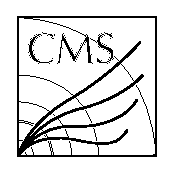
\includegraphics{cmslogo.eps}}
    \caption{Figure inserted by 
      \tt $\backslash$resizebox\{3cm\}\{!\}\{$\backslash$includegraphics\{cmslogo.eps\}\}.}
    \label{fig:ex1}
  \end{center}
\end{figure}

\begin{figure}[hbtp]
  \begin{center}
    \resizebox{5cm}{1cm}{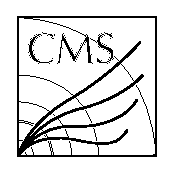
\includegraphics{cmslogo.eps}}
    \caption{Figure inserted by 
       \tt $\backslash$resizebox\{5cm\}\{1cm\}\{$\backslash$includegraphics\{cmslogo.eps\}\}.}
    \label{fig:ex2}
  \end{center}
\end{figure}

Quite often it is convenient to place 2 figures side by side as a single
floating body. An environment {\em 2figures} is provided for that
(see Fig.~\ref{fig:ex3} and \ref{fig:ex4}).

\begin{2figures}{hbtp}
  \resizebox{\linewidth}{0.5\linewidth}{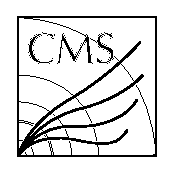
\includegraphics{cmslogo.eps}} &
  \resizebox{\linewidth}{0.5\linewidth}{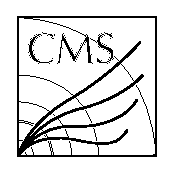
\includegraphics{cmslogo.eps}} \\
%  \resizebox{\linewidth}{!}{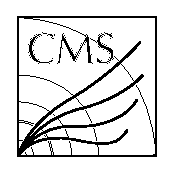
\includegraphics{cmslogo.eps}} &
%  \resizebox{\linewidth}{!}{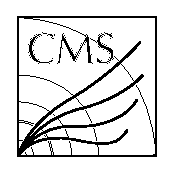
\includegraphics{cmslogo.eps}} \\
  \caption{The left figure}
  \label{fig:ex3} &
  \caption{The right figure}
  \label{fig:ex4} \\
\end{2figures}

%------------------------------------------------------------------------------

\section{Submitting a note}

Please follow the rules and procedures defined on the CMSDOC server, or request them by e-mail to:\begin{center} {\em cmsnotes@cmsdoc.cern.ch} \end{center}

\section{Reference example}

References should be placed at the end of the note 
(see example \cite{NOTE000}).

\begin{thebibliography}{9}
  \bibitem {NOTE000} {\bf CMS Note 2005/000},
    X.Somebody et al.,
    {\em "CMS Note Template"}.
\end{thebibliography}
 
%------------------------------------------------------------------------------
\pagebreak

{\small \begin{flushleft}
Appendix: A4/US page set-up\\
-1 - - - - - - - - - - - - - - - - - - - - - - - - - - - - - - - - - - - - - -\\
-2 - - - - - - - - - - - - - - - - - - - - - - - - - - - - - - - - - - - - - -\\
-3		See section 2.1\\
-4 - - - - - - - - - - - - - - - - - - - - - - - - - - - - - - - - - - - - - -\\
-5 - - - - - - - - - - - - - - - - - - - - - - - - - - - - - - - - - - - - - -\\
-6 - - - - - - - - - - - - - - - - - - - - - - - - - - - - - - - - - - - - - -\\
-7 - - - - - - - - - - - - - - - - - - - - - - - - - - - - - - - - - - - - - -\\
-8 - - - - - - - - - - - - - - - - - - - - - - - - - - - - - - - - - - - - - -\\
-9 - - - - - - - - - - - - - - - - - - - - - - - - - - - - - - - - - - - - - -\\
10 - - - - - - - - - - - - - - - - - - - - - - - - - - - - - - - - - - - - - -\\
-1 - - - - - - - - - - - - - - - - - - - - - - - - - - - - - - - - - - - - - -\\
-2 - - - - - - - - - - - - - - - - - - - - - - - - - - - - - - - - - - - - - -\\
-3 - - - - - - - - - - - - - - - - - - - - - - - - - - - - - - - - - - - - - -\\
-4 - - - - - - - - - - - - - - - - - - - - - - - - - - - - - - - - - - - - - -\\
-5 - - - - - - - - - - - - - - - - - - - - - - - - - - - - - - - - - - - - - -\\
-6 - - - - - - - - - - - - - - - - - - - - - - - - - - - - - - - - - - - - - -\\
-7 - - - - - - - - - - - - - - - - - - - - - - - - - - - - - - - - - - - - - -\\
-8 - - - - - - - - - - - - - - - - - - - - - - - - - - - - - - - - - - - - - -\\
-9 - - - - - - - - - - - - - - - - - - - - - - - - - - - - - - - - - - - - - -\\
20 - - - - - - - - - - - - - - - - - - - - - - - - - - - - - - - - - - - - - -\\
-1 - - - - - - - - - - - - - - - - - - - - - - - - - - - - - - - - - - - - - -\\
-2 - - - - - - - - - - - - - - - - - - - - - - - - - - - - - - - - - - - - - -\\
-3 - - - - - - - - - - - - - - - - - - - - - - - - - - - - - - - - - - - - - -\\
-4 - - - - - - - - - - - - - - - - - - - - - - - - - - - - - - - - - - - - - -\\
-5 - - - - - - - - - - - - - - - - - - - - - - - - - - - - - - - - - - - - - -\\
-6 - - - - - - - - - - - - - - - - - - - - - - - - - - - - - - - - - - - - - -\\
-7 - - - - - - - - - - - - - - - - - - - - - - - - - - - - - - - - - - - - - -\\
-8 - - - - - - - - - - - - - - - - - - - - - - - - - - - - - - - - - - - - - -\\
-9 - - - - - - - - - - - - - - - - - - - - - - - - - - - - - - - - - - - - - -\\
30 - - - - - - - - - - - - - - - - - - - - - - - - - - - - - - - - - - - - - -\\
-1 - - - - - - - - - - - - - - - - - - - - - - - - - - - - - - - - - - - - - -\\
-2 - - - - - - - - - - - - - - - - - - - - - - - - - - - - - - - - - - - - - -\\
-3 - - - - - - - - - - - - - - - - - - - - - - - - - - - - - - - - - - - - - -\\
-4 - - - - - - - - - - - - - - - - - - - - - - - - - - - - - - - - - - - - - -\\
-5 - - - - - - - - - - - - - - - - - - - - - - - - - - - - - - - - - - - - - -\\
-6 - - - - - - - - - - - - - - - - - - - - - - - - - - - - - - - - - - - - - -\\
-7 - - - - - - - - - - - - - - - - - - - - - - - - - - - - - - - - - - - - - -\\
-8 - - - - - - - - - - - - - - - - - - - - - - - - - - - - - - - - - - - - - -\\
-9 - - - - - - - - - - - - - - - - - - - - - - - - - - - - - - - - - - - - - -\\
40 - - - - - - - - - - - - - - - - - - - - - - - - - - - - - - - - - - - - - -\\
-1 - - - - - - - - - - - - - - - - - - - - - - - - - - - - - - - - - - - - - -\\
-2 - - - - - - - - - - - - - - - - - - - - - - - - - - - - - - - - - - - - - -\\
-3 - - - - - - - - - - - - - - - - - - - - - - - - - - - - - - - - - - - - - -\\
-4 - - - - - - - - - - - - - - - - - - - - - - - - - - - - - - - - - - - - - -\\
-5 - - - - - - - - - - - - - - - - - - - - - - - - - - - - - - - - - - - - - -\\
-6 - - - - - - - - - - - - - - - - - - - - - - - - - - - - - - - - - - - - - -\\
-7 - - - - - - - - - - - - - - - - - - - - - - - - - - - - - - - - - - - - - -\\
-8 - - - - - - - - - - - - - - - - - - - - - - - - - - - - - - - - - - - - - -\\
-9 - - - - - - - - - - - - - - - - - - - - - - - - - - - - - - - - - - - - - -\\
50 - - - - - - - - - - - - - - - - - - - - - - - - - - - - - - - - - - - - - -\\
-1 - - - - - - - - - - - - - - - - - - - - - - - - - - - - - - - - - - - - - -\\
-2 - - - - - - - - - - - - - - - - - - - - - - - - - - - - - - - - - - - - - -\\
-3 - - - - - - - - - - - - - - - - - - - - - - - - - - - - - - - - - - - - - -\\
-4 - - - - - - - - - - - - - - - - - - - - - - - - - - - - - - - - - - - - - -\\
-5 - - - - - - - - - - - - - - - - - - - - - - - - - - - - - - - - - - - - - -\\
-6 - - - - - - - - - - - - - - - - - - - - - - - - - - - - - - - - - - - - - -\\
-7 - - - - - - - - - - - - - - - - - - - - - - - - - - - - - - - - - - - - - -\\
-8 - - - - - - - - - - - - - - - - - - - - - - - - - - - - - - - - - - - - - -\\
-9 - - - - - - - - - - - - - - - - - - - - - - - - - - - - - - - - - - - - - -\\
60 - - - - - - - - - - - - - - - - - - - - - - - - - - - - - - - - - - - - - -\\
-1 - - - - - - - - - - - - - - - - - - - - - - - - - - - - - - - - - - - - - -\\
-2 - - - - - - - - - - - - - - - - - - - - - - - - - - - - - - - - - - - - - -\\
-3 - - - - - - - - - - - - - - - - - - - - - - - - - - - - - - - - - - - - - -\\
-4 - - - - - - - - - - - - - - - - - - - - - - - - - - - - - - - - - - - - - -\\
-5 - - - - - - - - - - - - - - - - - - - - - - - - - - - - - - - - - - - - - -\\
-6 - - - - - - - - - - - - - - - - - - - - - - - - - - - - - - - - - - - - - -\\
-7 - - - - - - - - - - - - - - - - - - - - - - - - - - - - - - - - - - - - - -\\
-8 - - - - - - - - - - - - - - - - - - - - - - - - - - - - - - - - - - - - - -\\
-9 - - - - - - - - - - - - - - - - - - - - - - - - - - - - - - - - - - - - - -\\
70 - - - - - - - - - - - - - - - - - - - - - - - - - - - - - - - - - - - - - -\\
-1 - - - - - - - - - - - - - - - - - - - - - - - - - - - - - - - - - - - - - -\\
-2 - - - - - - - - - - - - - - - - - - - - - - - - - - - - - - - - - - - - - -\\
-3 - - - - - - - - - - - - - - - - - - - - - - - - - - - - - - - - - - - - - -\\
-4 - - - - - - - - - - - - - - - - - - - - - - - - - - - - - - - - - - - - - -\\
-5 - - - - - - - - - - - - - - - - - - - - - - - - - - - - - - - - - - - - - -\\
-6 - - - - - - - - - - - - - - - - - - - - - - - - - - - - - - - - - - - - - -\\
-7 - - - - - - - - - - - - - - - - - - - - - - - - - - - - - - - - - - - - - -\\
-8 - - - - - - - - - - - - - - - - - - - - - - - - - - - - - - - - - - - - - -\\
-9 - - - - - - - - - - - - - - - - - - - - - - - - - - - - - - - - - - - - - -\\
80 - - - - - - - - - - - - - - - - - - - - - - - - - - - - - - - - - - - - - -\\
-1 - - - - - - - - - - - - - - - - - - - - - - - - - - - - - - - - - - - - - -\\
-2 - - - - - - - - - - - - - - - - - - - - - - - - - - - - - - - - - - - - - -\\
-3 - - - - - - - - - - - - - - - - - - - - - - - - - - - - - - - - - - - - - -\\
-4 - - - - - - - - - - - - - - - - - - - - - - - - - - - - - - - - - - - - - -\\
-5 - - - - - - - - - - - - - - - - - - - - - - - - - - - - - - - - - - - - - -\\
-6 - - - - - - - - - - - - - - - - - - - - - - - - - - - - - - - - - - - - - -\\
-7 - - - - - - - - - - - - - - - - - - - - - - - - - - - - - - - - - - - - - -\\
-8 - - - - - - - - - - - - - - - - - - - - - - - - - - - - - - - - - - - - - -\\
-9 - - - - - - - - - - - - - - - - - - - - - - - - - - - - - - - - - - - - - -\\
90 - - - - - - - - - - - - - - - - - - - - - - - - - - - - - - - - - - - - - -\\
-1 - - - - - - - - - - - - - - - - - - - - - - - - - - - - - - - - - - - - - -\\
-2 - - - - - - - - - - - - - - - - - - - - - - - - - - - - - - - - - - - - - -\\
-3 - - - - - - - - - - - - - - - - - - - - - - - - - - - - - - - - - - - - - -\\
-4 - - - - - - - - - - - - - - - - - - - - - - - - - - - - - - - - - - - - - -\\
-5 - - - - - - - - - - - - - - - - - - - - - - - - - - - - - - - - - - - - - -\\
-6 - - - - - - - - - - - - - - - - - - - - - - - - - - - - - - - - - - - - - -\\
-7 - - - - - - - - - - - - - - - - - - - - - - - - - - - - - - - - - - - - - -\\
-8 - - - - - - - - - - - - - - - - - - - - - - - - - - - - - - - - - - - - - -\\
-9 - - - - - - - - - - - - - - - - - - - - - - - - - - - - - - - - - - - - - -\\
100- - - - - - - - - - - - - - - - - - - - - - - - - - - - - - - - - - - - - -\\
\end{flushleft} }

\end{document}
